\section{Jak dlouhé je pobřeží Velké Británie?}\label{sec:pobrezi_velke_britanie}
Položme si na začátek trochu jinou otázku, kterou si z počátku položil i Benoit Mandelbrot: \emph{Jaká je podstata tvaru pobřeží?} Ta se stala podstatnou v jeho práci \emph{"How Long Is the Coast of Britain?"}. Uvažme část pobřeží s počátečním a koncovým bodem (viz obrázek \ref{fig:pobrezi}).
\begin{figure}[h]
    \centering
    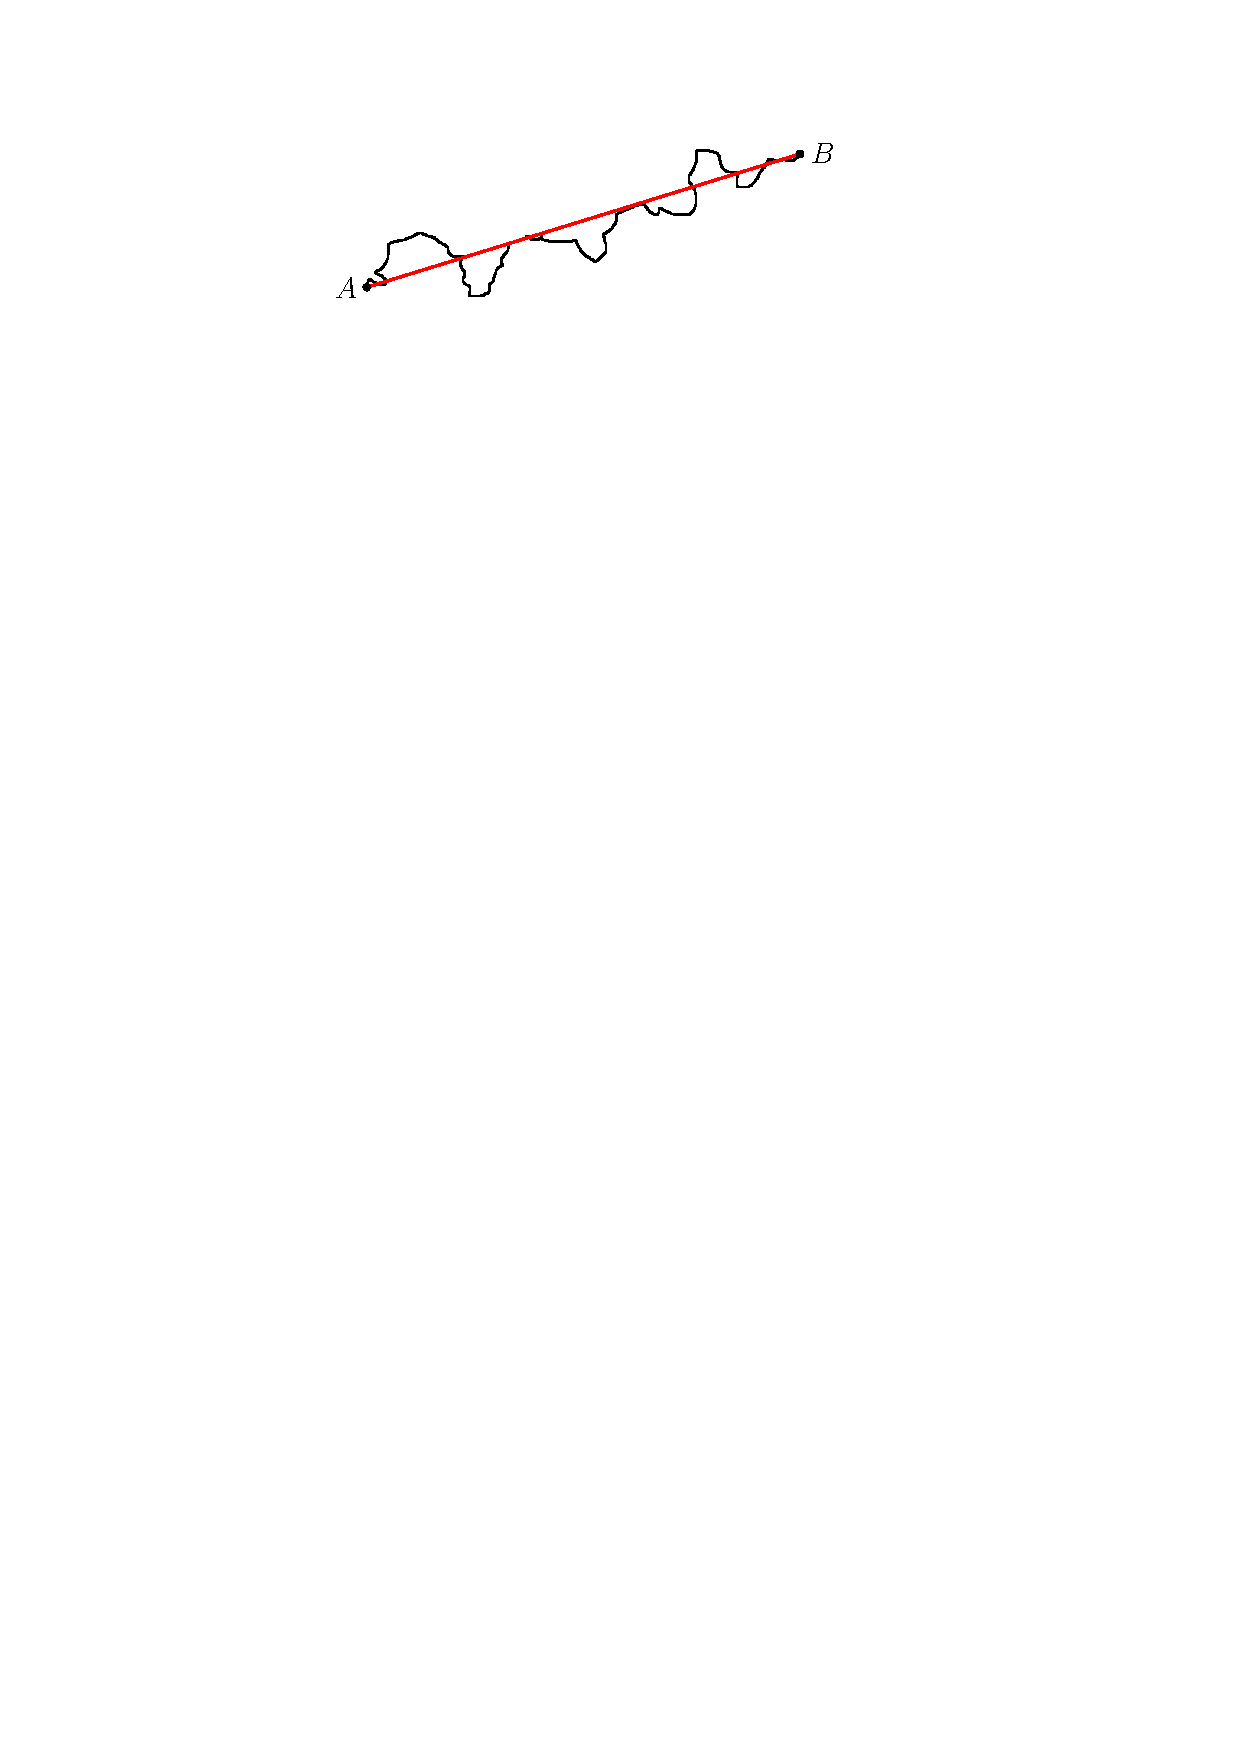
\includegraphics[scale=\normalipe]{ch01_pobrezi.pdf}
    \caption{Příklad mapy pobřeží se spojnicí bodů $A$ a $B$.}
    \label{fig:pobrezi}
\end{figure}
Zjevně jeho délka je zdola omezena délkou spojnice koncových bodů $A$ a $B$, nicméně typické pobřeží je velmi nepravidelné a klikaté, a jeho skutečná délka je tak často mnohem delší než délka spojnice jeho koncových bodů. Existují různé metody, které nám umožňují určit přesněji jeho délku. V této části si dovolím se odkázat na knihu \citep[str. 79]{Mandelbrot1983}, kde je problematika detailněji popsána.\par
Vyjasněme si zde nejdříve pár bodů. Pobřeží, které zkoumáme, má pevné hranice (tj. zanedbáváme např. přílivy a odlivy nastávající během roku), a dále jsme schopni rozlišovat libovolně krátké vzdálenosti.\par
Mějme zadané libovolné měřítko mapy $\varepsilon>0$. Podél pobřeží začneme umisťovat tyče tak, že po každém umístění provedeme na mapě krok, přičemž začínáme v bodě $A$ a postupujeme až k budu $B$ (popř. pokud měříme délku pobřeží ostrova, pokračujeme dokud se nevrátíme tam, kde jsme začali). Předpokládejme, že jsme provedli celkově $n$ kroků (zde je důležité si uvědomit, ). \emph{Přibližnou délku pobřeží} $\ell(\varepsilon)$ pro zadané měřítko pak stanovíme jako
\begin{equation*}
    \ell(\varepsilon)=n\cdot\varepsilon.
\end{equation*}
\begin{figure}[h]
    \centering
    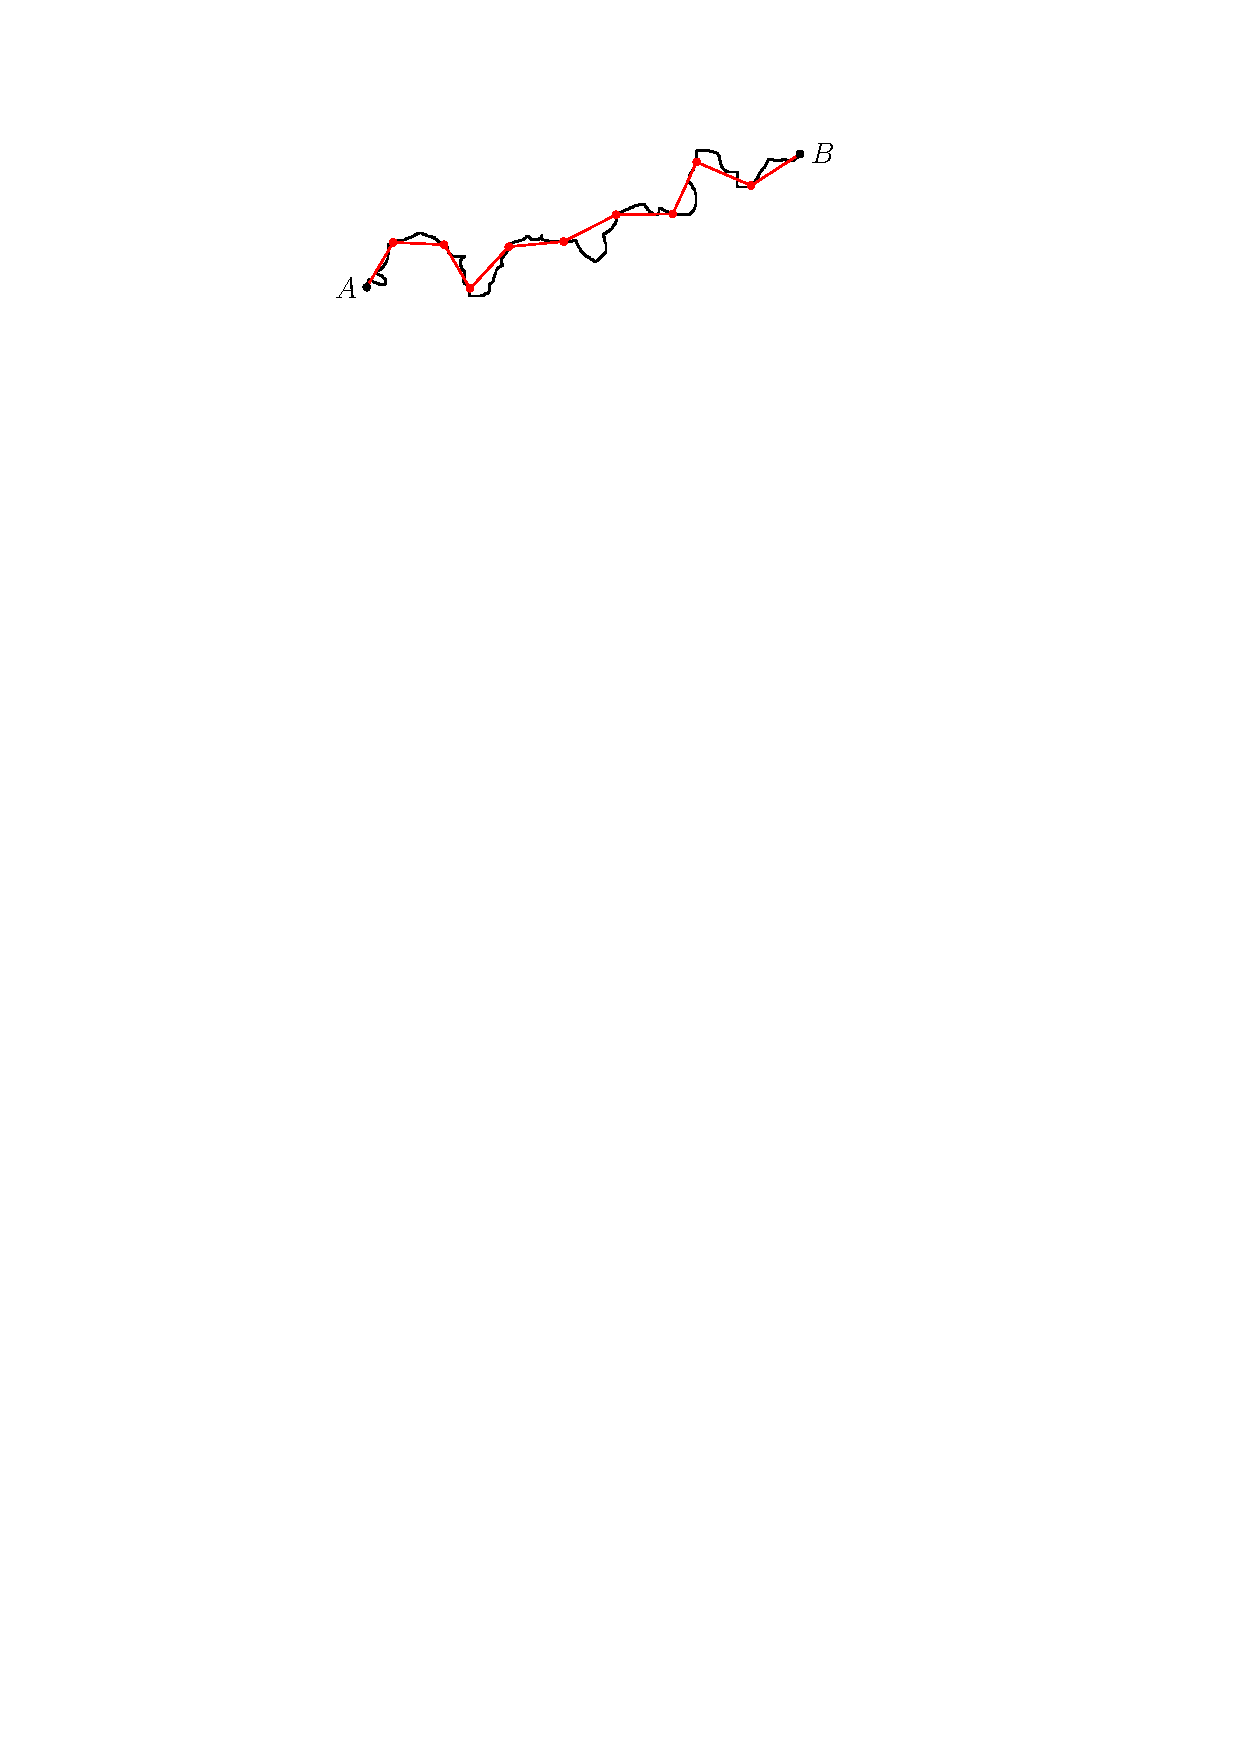
\includegraphics[scale=\normalipe]{ch01_pobrezi_aproximace.pdf}
    \caption{Odhad délky pobřeží, kde $n=10$ při zvoleném $\varepsilon$.}
    \label{fig:pobrezi_aproximace}
\end{figure}
Nyní by nás mohlo napadnout, že pro zmenšující se $\varepsilon$, tj. $\varepsilon\to0$, bude hodnota $\ell(\varepsilon)$ konvergovat ke skutečné délce pobřeží. Tzn. označíme-li skutečnou délku pobřeží $L$, pak bychom mohli očekávat, že platí
\begin{equation}\label{eq:aproximace_limita}
    L=\lim_{\varepsilon\to0}{\ell(\varepsilon)}.
\end{equation}
Jenže, bohužel, rovnost \eqref{eq:aproximace_limita} ve skutečnosti neplatí. Proč? Je třeba si uvědomit, že zde pracujeme s \emph{mapou}, která má určité \emph{měřítko}. Pokud bychom měli pobřeží na mapě s měřítkem $1\,:\,100\;000$ ($\varepsilon=10^5$), uvidíme méně detailů, než kdybychom jej zkoumali na mapě s měřítkem $1\,:\,1\;000$ ($\varepsilon=10^3$). (Viz obrázek \ref{fig:pobrezi_zoom}.)\par
\begin{figure}[h]
    \centering
    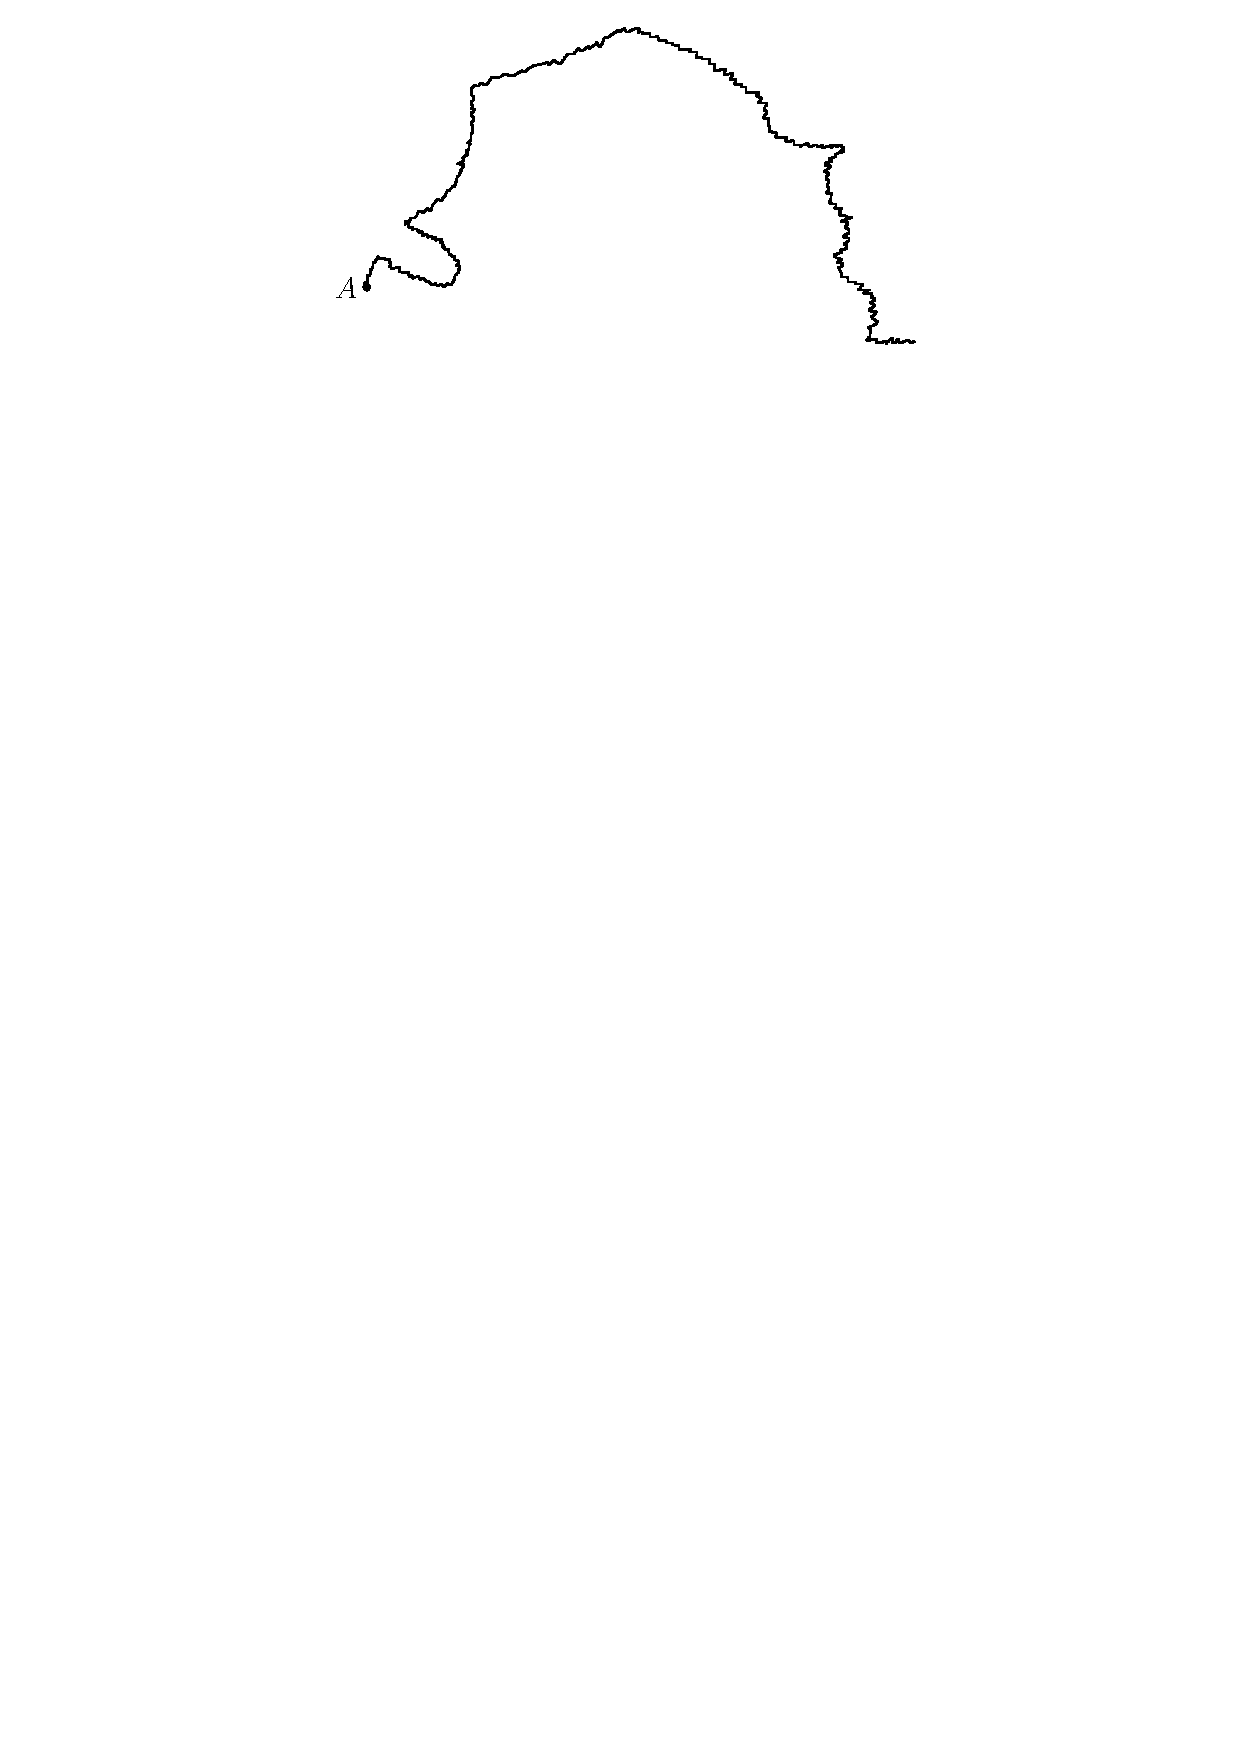
\includegraphics[scale=\normalipe]{ch01_pobrezi_zoom.pdf}
    \caption{Část pobřeží od bodu $A$ v menším měřítku.}
    \label{fig:pobrezi_zoom}
\end{figure}
Nově odhalené detaily (menší poloostrůvky apod.) zde přispívají k celkové délce pobřeží $\ell(\varepsilon)$. Postupným zmenšováním měřítka mapy bychom tak odhalili další detaily. Naše původní idea tak selhává, neboť pro $\varepsilon\to0$ hodnota $\ell(\varepsilon)$ poroste nade všechny meze, tj. $\lim_{\varepsilon\to0}{\ell(\varepsilon)}=\infty$.\par
Nabízí se otázka: Proč se toto děje? Pokud se ohlédneme zpět za Eukleidovskou geometrií, tento problém zde nenastává. Např. kružnice v eukleidovské rovině $\mathbb{E}_2$ změnou měřítka žádné další detaily křivky neobjevíme (podobně u jiných geometrických útvarů, viz obrázky \ref{subfig:kruznice} a \ref{subfig:kruznice_zoom}). 
\begin{figure}[h]
    \centering
    \begin{subfigure}{\subfigwidth}
        \centering
        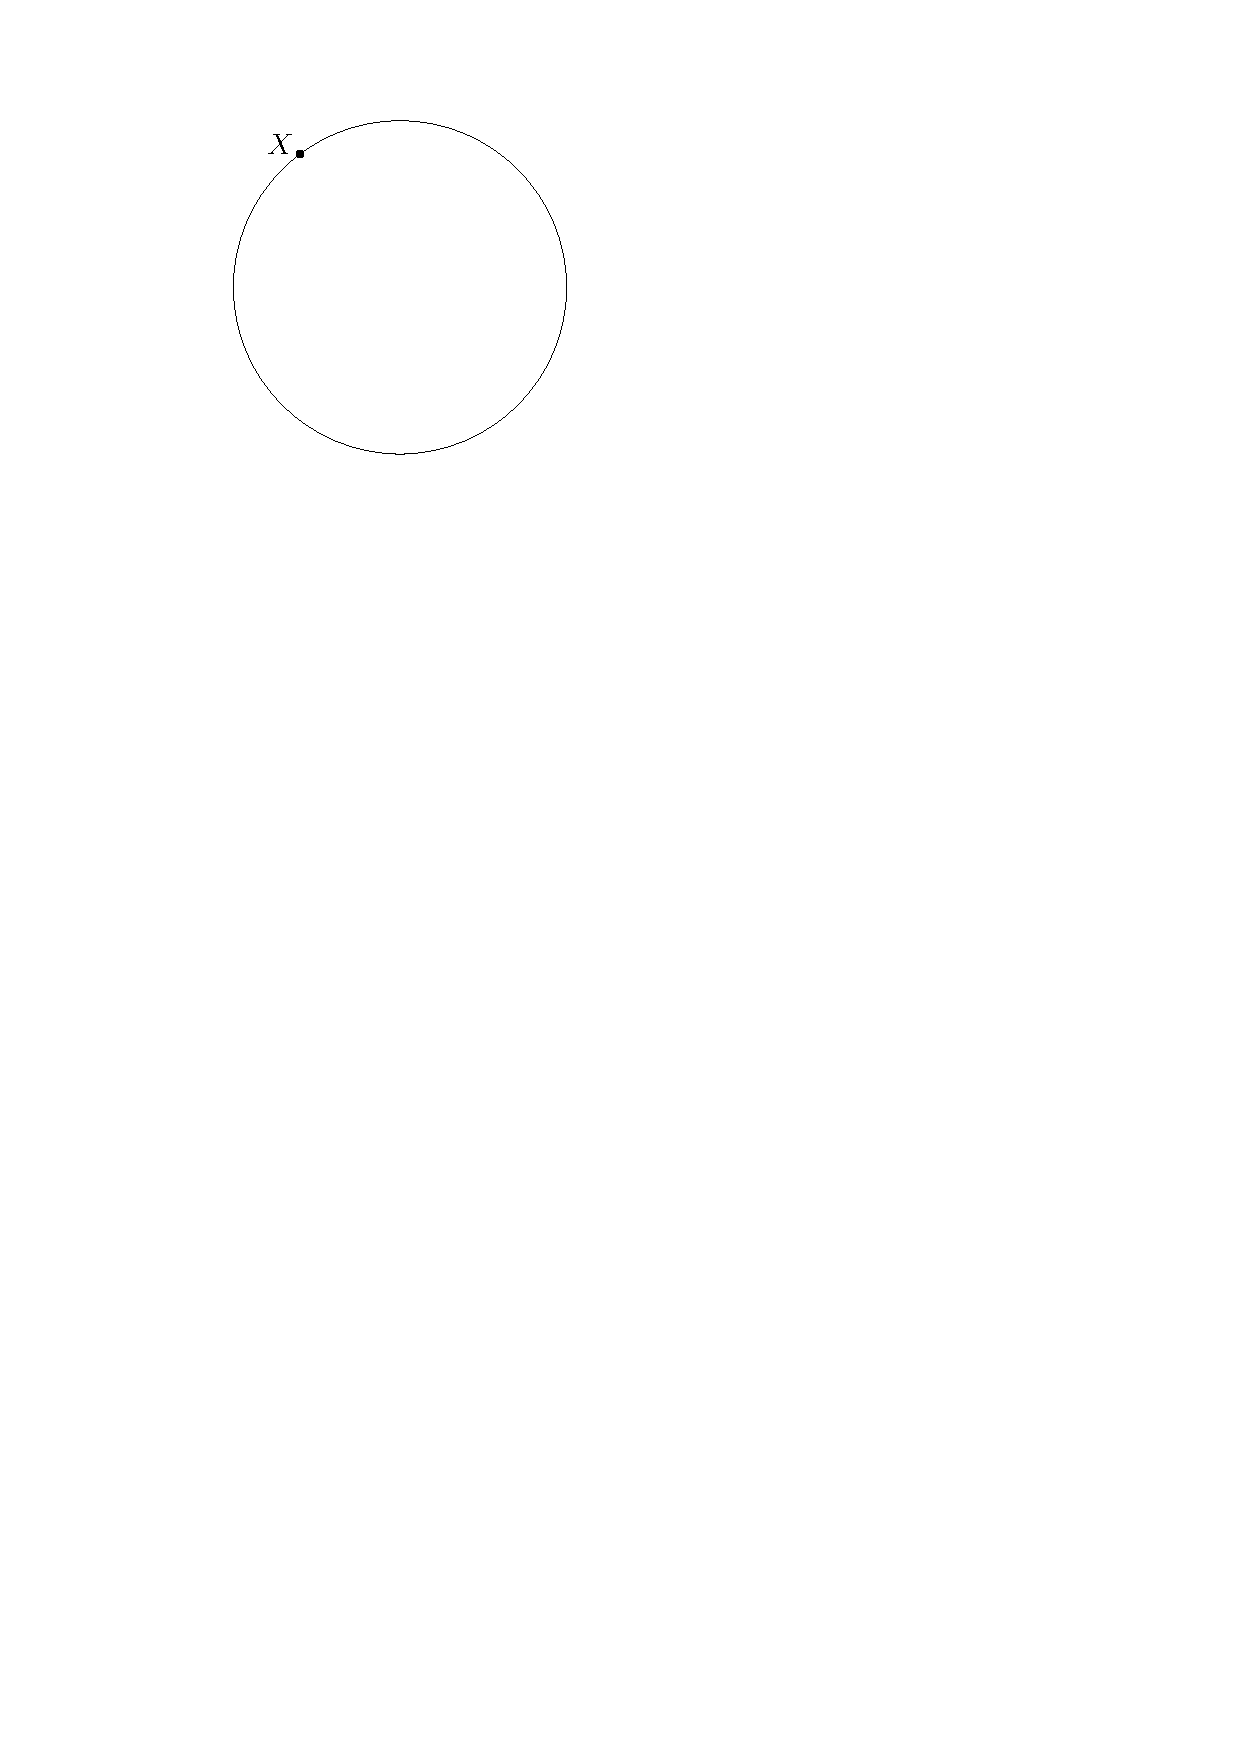
\includegraphics[scale=\normalipe]{ch01_kruznice.pdf}
        \caption{Kružnice v menším měřítku.}
        \label{subfig:kruznice}
    \end{subfigure}
    \quad
    \begin{subfigure}{\subfigwidth}
        \centering
        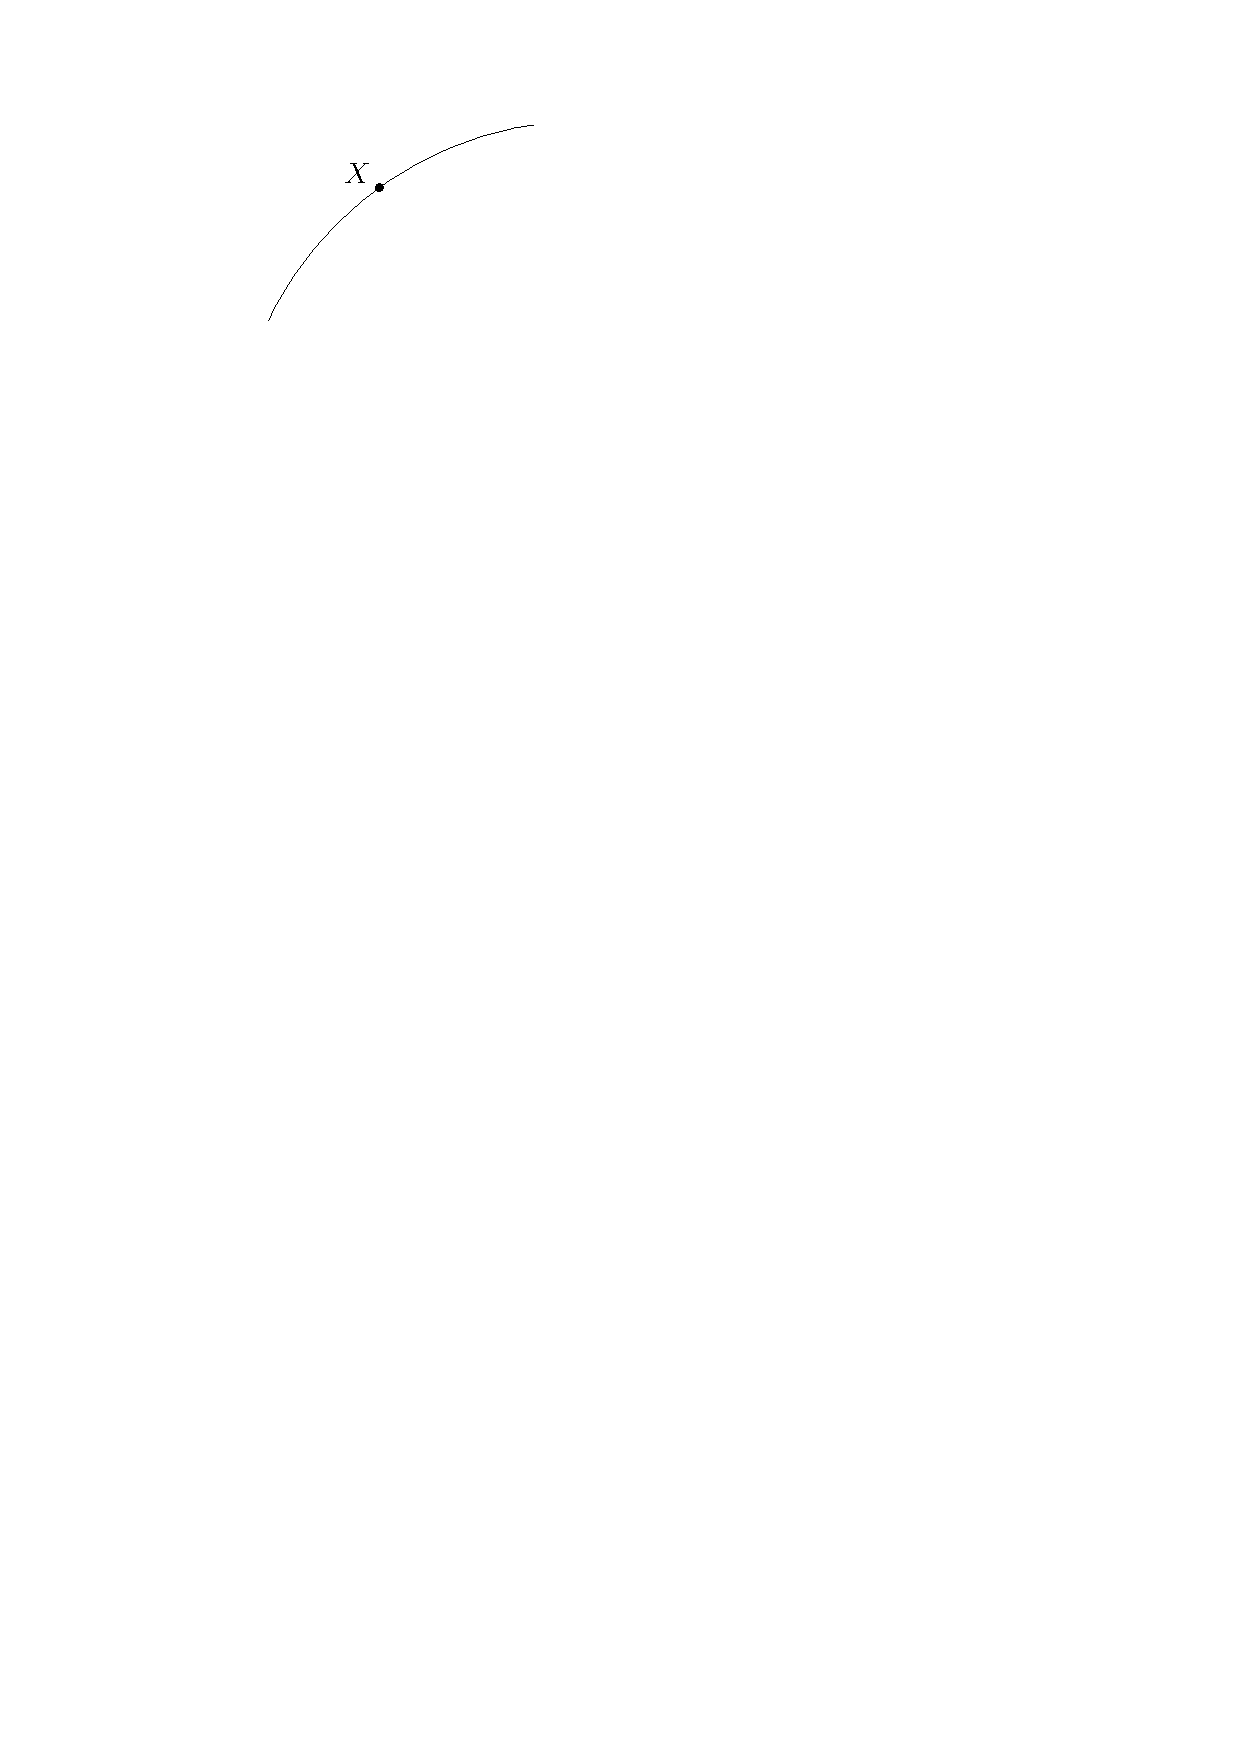
\includegraphics[scale=\normalipe]{ch01_kruznice_zoom.pdf}
        \caption{Část kružnice ve větším měřítku.}
        \label{subfig:kruznice_zoom}
    \end{subfigure}
\end{figure}
Díky tomu můžeme v případě počítání obvodu kružnice použít např. Archimédovu metodu (tj. postupnou aproximaci obvodu pomocí $n$-úhelníků). V konečném důsledku tak obdržíme limitu
\begin{equation*}
    O=\lim_{n\to\infty}{2\pi\cdot r\cdot\sin{\dfrac{\pi}{n}}},
\end{equation*}
která konverguje k $2\pi r$, kde $r$ je poloměr kružnice.\par
